\documentclass[sigconf]{acmart}
\usepackage{algorithm}
\usepackage{caption}
\usepackage{todonotes}
\usepackage{algorithmicx}
\usepackage[noend]{algpseudocode}

%%
%% \BibTeX command to typeset BibTeX logo in the docs
\AtBeginDocument{%
  \providecommand\BibTeX{{%
    \normalfont B\kern-0.5em{\scshape i\kern-0.25em b}\kern-0.8em\TeX}}}

%% Rights management information.  This information is sent to you
%% when you complete the rights form.  These commands have SAMPLE
%% values in them; it is your responsibility as an author to replace
%% the commands and values with those provided to you when you
%% complete the rights form.
\setcopyright{acmcopyright}
\copyrightyear{2018}
\acmYear{2018}
\acmDOI{10.1145/1122445.1122456}

%% These commands are for a PROCEEDINGS abstract or paper.
\acmConference[Woodstock '18]{Woodstock '18: ACM Symposium on Neural
  Gaze Detection}{June 03--05, 2018}{Woodstock, NY}
\acmBooktitle{Woodstock '18: ACM Symposium on Neural Gaze Detection,
  June 03--05, 2018, Woodstock, NY}
\acmPrice{15.00}
\acmISBN{978-1-4503-XXXX-X/18/06}


%%
%% Submission ID.
%% Use this when submitting an article to a sponsored event. You'll
%% receive a unique submission ID from the organizers
%% of the event, and this ID should be used as the parameter to this command.
%%\acmSubmissionID{123-A56-BU3}

%%
%% The majority of ACM publications use numbered citations and
%% references.  The command \citestyle{authoryear} switches to the
%% "author year" style.
%%
%% If you are preparing content for an event
%% sponsored by ACM SIGGRAPH, you must use the "author year" style of
%% citations and references.
%% Uncommenting
%% the next command will enable that style.
%%\citestyle{acmauthoryear}

%%
%% end of the preamble, start of the body of the document source.
\begin{document}

%%
%% The "title" command has an optional parameter,
%% allowing the author to define a "short title" to be used in page headers.
\title{Context-Free Path Queries, Planar Graphs and Friends}
 
%%
%% The "author" command and its associated commands are used to define
%% the authors and their affiliations.
%% Of note is the shared affiliation of the first two authors, and the
%% "authornote" and "authornotemark" commands
%% used to denote shared contribution to the research.

\author{Alexandra Istomina}
\affiliation{%
  \institution{Saint-Petersburg State University}
  \city{Saint-Petersburg}
  \country{Russia}
 }

\author{Alexandra Olemskaya}
\affiliation{%
  \institution{Inria Paris-Rocquencourt}
  \city{Rocquencourt}
  \country{France}
}

\author{Ekaterina Shemetova}
\affiliation{%
  \institution{Inria Paris-Rocquencourt}
  \city{Rocquencourt}
  \country{France}
}


\author{Semyon Grigorev}
\affiliation{%
 \institution{Rajiv Gandhi University}
 \streetaddress{Rono-Hills}
 \city{Doimukh}
 \state{Arunachal Pradesh}
 \country{India}}



%%
%% By default, the full list of authors will be used in the page
%% headers. Often, this list is too long, and will overlap
%% other information printed in the page headers. This command allows
%% the author to define a more concise list
%% of authors' names for this purpose.

%%
%% The abstract is a short summary of the work to be presented in the
%% article.
\begin{abstract}

Abstract is very abstract.

\end{abstract}

%%
%% The code below is generated by the tool at http://dl.acm.org/ccs.cfm.
%% Please copy and paste the code instead of the example below.
%%
\begin{CCSXML}
<ccs2012>
 <concept>
  <concept_id>10010520.10010553.10010562</concept_id>
  <concept_desc>Computer systems organization~Embedded systems</concept_desc>
  <concept_significance>500</concept_significance>
 </concept>
 <concept>
  <concept_id>10010520.10010575.10010755</concept_id>
  <concept_desc>Computer systems organization~Redundancy</concept_desc>
  <concept_significance>300</concept_significance>
 </concept>
 <concept>
  <concept_id>10010520.10010553.10010554</concept_id>
  <concept_desc>Computer systems organization~Robotics</concept_desc>
  <concept_significance>100</concept_significance>
 </concept>
 <concept>
  <concept_id>10003033.10003083.10003095</concept_id>
  <concept_desc>Networks~Network reliability</concept_desc>
  <concept_significance>100</concept_significance>
 </concept>
</ccs2012>
\end{CCSXML}

\ccsdesc[500]{Computer systems organization~Embedded systems}
\ccsdesc[300]{Computer systems organization~Redundancy}
\ccsdesc{Computer systems organization~Robotics}
\ccsdesc[100]{Networks~Network reliability}

%%
%% Keywords. The author(s) should pick words that accurately describe
%% the work being presented. Separate the keywords with commas.
\keywords{datasets, neural networks, gaze detection, text tagging}


%%
%% This command processes the author and affiliation and title
%% information and builds the first part of the formatted document.
\maketitle
\section{Introduction}


Language-constrained path querying~\cite{barrett2000formal} is a technique for graph navigation querying.
This technique allows one to use formal languages as constraints on paths in edge-labeled graphs: path satisfies constraints if labels along it form a word from the specified language.

The utilization of regular languages as constraints, or \textit{Regular Path Querying} (RPQ), is most well-studied and widespread.
Different aspects of RPQs are actively studied in graph databases~\cite{10.1145/2463664.2465216, 10.1145/3104031,10.1145/2850413}, while regular constraints are supported in such popular query languages as PGQL~\cite{10.1145/2960414.2960421} and SPARQL\footnote{Specification of regular constraints in SPARQL property paths: \url{https://www.w3.org/TR/sparql11-property-paths/}. Access date: 07.07.2020.}~\cite{10.1007/978-3-319-25007-6_1} (property paths).
Nevertheless, there is certainly room for improvement of RPQ efficiency, and new solutions are being created~\cite{Wang2019,10.1145/2949689.2949711}.

At the same time, using more powerful languages, namely context-free languages, as constraints has gained popularity in the last few years.
\textit{Context-Free Path Querying} problem (CFPQ) was introduced by Mihalis Yannakakis in 1990 in~\cite{Yannakakis}.
Many algorithms were proposed since that time, but recently, Jochem Kuijpers et al. showed in~\cite{Kuijpers:2019:ESC:3335783.3335791} that state-of-the-art CFPQ algorithms are not performant enough for practical use.
This motivates us to develop new algorithms for CFPQ.

One promising way to achieve high-performance solutions for graph analysis problems is to reduce them to linear algebra operations.
This way, GraphBLAS~\cite{7761646} API, the description of basic linear algebra primitives, was proposed.
Solutions that use libraries that implement this API, such as SuiteSparce~\cite{10.1145/3322125} and CombBLAS~\cite{10.1177/1094342011403516}, show that reduction to linear algebra is a way to utilize high-performance parallel and distributed computations for graph analysis.

Rustam Azimov shows in~\cite{Azimov:2018:CPQ:3210259.3210264} how to reduce CFPQ to matrix multiplication.
Later, it was shown in~\cite{Mishin:2019:ECP:3327964.3328503} and~\cite{10.1145/3398682.3399163} that utilization of appropriate libraries for linear algebra for Azimov's algorithm implementation makes a practical solution for CFPQ.
However Azimov's algorithm requires transforming the input grammar to Chomsky Normal Form, which leads to the grammar size increase, and hence worsens performance, especially for regular queries and complex context-free queries.

To solve these problems, an algorithm based on automata intersection was proposed~\cite{10.1007/978-3-030-54832-2_6}.
This algorithm is based on linear algebra and does not require the transformation of the input grammar.
We improve the algorithm in this work.
We reduce the above mentioned solution to operations over Boolean matrices, thus simplifying its description and implementation.
Also, we show that this algorithm is performant enough for regular queries, so it is a good candidate for integration with real-world query languages: one algorithm can be used to evaluate both regular and context-free queries.

Moreover, we show that this algorithm opens the way to tackle a long-standing problem about the existence of truly-subcubic $O(n^{3-\epsilon})$ CFPQ algorithm ~\cite{10.1145/1328438.1328460, Yannakakis}.
Currently, the best result is an $O(n^3/\log{n})$ algorithm of Swarat Chaudhuri~\cite{10.1145/1328438.1328460}.
Also, there exist truly subcubic solutions which use fast matrix multiplication for some fixed subclasses of context-free languages~\cite{8249039}.
Unfortunately, this solutions cannot be generalized to arbitrary CFPQs.
In this work, we identify incremental transitive closure as a bottleneck on the way to achieve subcubic time complexity for CFPQ.

To sum up, we make the following contributions.
\begin{enumerate}
	\item We rethink and improve the CFPQ algorithm based on tensor-product proposed by Orachev et al. ~\cite{10.1007/978-3-030-54832-2_6}.
	We reduce this algorithm to operations over Boolean matrices.
	As a result, all-path query semantics is handled, as opposed to the previous matrix-based solution which handles only the single-path semantics.
	Also, both regular and context-free grammars can be used as queries.
	We prove the correctness and time complexity for the proposed algorithm.
	\item We demonstrate the interconnection between CFPQ and incremental transitive closure.
	We show that incremental transitive closure is a bottleneck on the way to achieve faster CFPQ algorithm for general case of arbitrary graphs as well as for special families of graphs, such as planar graphs.
	\item We implement the described algorithm and evaluate it on real-world data for both RPQ and CFPQ. Results show that the proposed solution is comparable with existing solutions for CFPQ and RPQ, thus it is a promising way to create a unified algorithm for both CFPQ and RPQ evaluation.
\end{enumerate}
\section{Preliminaries}
\label{sec:prel}
\label{preliminaries}
\paragraph{Formal languages.} 
A \textit{context-free grammar} is a 4-tuple $G = (\Sigma, N, P, S)$, where $\Sigma$ is a finite set of alphabet symbols,  $N$ is a set of nonterminal symbols, $P$ is a set of production rules and $S$ is a start nonterinal. $L(G)$ is a context-free language generated by context-free grammar $G$. We use the notation $A \stackrel {*}{\Rightarrow } w$  to denote that the string $w \in \Sigma^*$ can be derived from a nonterminal $A$ by sequence of applying the production rules from $P$. A \textit{parse tree} is an entity which represents the structure of the derivation of a terminal string from some nonterminal.


A grammar $G$ is said to be is in the \textit{Chomsky normal form}, if all production rules of $P$ are of the form:
$A \rightarrow BC$, $A \rightarrow a$ or $S \rightarrow \varepsilon$, where $A, B, C \in N$ and $a \in \Sigma$. 


The set of all context-free languages is identical to the set of languages accepted by pushdown automata (PDA). \textit{Pushdown automaton} is a 7-tuple $M = (Q, \Sigma, \Gamma, \delta, q_0, Z, F)$, where $Q$ is a finite set of states, $\Sigma$ is a input alphabet, $\Gamma$ is a finite set which is called the stack alphabet, $\delta$ is a finite subset of $Q \times (\Sigma \cap \{\varepsilon\}) \times \Gamma \times Q \times \Gamma^*$,
$q_{0}\in Q$ is the start state, $Z \in \Gamma$ is the initial stack symbol and
$F\subseteq Q$ is the set of accepting states.


A \textit{regular language} is a language that can be expressed with a regular expression or a deterministic or non-deterministic finite automata.
A \textit{nondeterministic finite automaton} (NFA) is represented by a 5-tuple, $(Q,\Sigma ,\delta ,Q_{0},F)$, where $Q$ is a finite set of states, $\Sigma$ is a finite set of input symbols, $\delta:Q\times \Sigma \rightarrow 2^{|Q|}$ is a transition function, $Q_0 \subseteq Q$ is a set of inial states, $F \subseteq Q$ is a set of accepting (final) states. \textit{Deterministic finite automaton} is a NFA with the following restrictions: each of its transitions is uniquely determined by its source state and input symbol, and reading an input symbol is required for each state transition.


 For a language $L$ over an alphabet $\Sigma$, its rational index $\rho_L$ is a function defined as follows:
$$\rho_L(n) = \max\{\min\{|w|:w \in L \cap K\}, K \in {Rat}_n, L \cap K \neq \emptyset\},$$ where $|w|$ is the length of a word $w$ and ${Rat}_n$ denotes the set of regular languages on an alphabet $\Sigma$, recognized by a finite nondeterministic automation with at most $n$ states.
\paragraph{Bounded-oscillation languages.} 
Oscillation is defined using a hierarchy of \textit{harmonics}. Let $\bar{a}$ be a \textit{push}-move and $a$ be a \textit{pop}-move. Then a PDA run $r$ can be described by a well-nested sequence $\alpha(r)$ of $\bar{a}$-s and $a$-s. Two positions $i<j$ form a \textit{matching pair} if the corresponding $\bar{a}$ at $i$-th position of the sequence matches with $a$ at $j$-th position. For example, word $\bar{a}\bar{a}\bar{a}aa\bar{a}aa$ has the following set of matching pairs: $\{(1, 8), (2, 5), (3, 4), (6, 7)\}$ ($\bar{a}(\bar{a}(\bar{a}a)a)(\bar{a}a)a$).


Harmonics are inductively defined as follows:
\begin{itemize}
\item  order 0 harmonic $h_0$ is $\varepsilon$
\item  $h_{(i+1)}$ harmonic is $\bar{a}h_ia\ \bar{a}h_ia$.
\end{itemize}
\begin{figure}
\centering
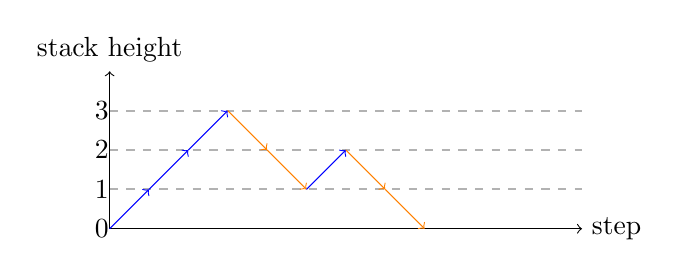
\begin{tikzpicture}
    \draw[thick, dashed, opacity=0.3] (0,0.5) -- (6,0.5);
     \draw[thick, dashed, opacity=0.3] (0,1) -- (6,1);
      \draw[thick, dashed, opacity=0.3] (0,1.5) -- (6,1.5);
      \draw[->] (0,0) -- (6,0) node[right] {step};
      \draw[->] (0,0) -- (0,2) node[above] {stack height};
     \draw[->, blue] (0,0) -- (0.5,0.5);
      \draw[->, blue] (0.5,0.5) -- (1,1);
      \draw[->, blue] (1,1) -- (1.5,1.5);
       \draw[->, orange] (1.5,1.5) -- (2,1);
    \draw[->, orange] (2,1) -- (2.5,0.5);
    \draw[->, blue] (2.5,0.5) -- (3,1);
    \draw[->, orange] (3,1) -- (3.5,0.5);
 \draw[->, orange] (3.5,0.5) -- (4,0);
\node (null) at (-0.1, 0) {0}; 
\node (one) at (-0.1, 0.5) {1}; 
\node (two) at (-0.1, 1) {2}; 
\node (three) at (-0.1, 1.5) {3}; 
    \end{tikzpicture}
\caption{Stack heights during the run of PDA.}
\label{oscb}
\end{figure}


PDA run $r$ is \textit{k-oscillating} if the harmonic of order $k$ is the greatest harmonic that occurs in $r$ after removing $0$ or more matching pairs. \textit{Bounded-oscillation languages} are languages accepted by pushdown automata with all runs $k$-oscillating. It is important that the problem whether a given CFL is a bounded-oscillation language is undecidable \cite{BoundOsc}.
\begin{example}
Consider Figure \ref{oscb}. It shows how the stack height changes during the run of a PDA. Corresponding well-nested word $\alpha(r)$ is $\bar{a}\bar{a}\bar{a}aa\bar{a}aa$. The greatest harmonic in this word is order 1 harmonic (moves forming harmonic are marked in bold, removed matching pairs are $(1, 8)$ and $(2, 5)$): $\bar{a}\bar{a}\mathbf{\bar{a}a}a\mathbf{\bar{a}a}a$, therefore oscillation of the run $r$ is 1.
\end{example}


The oscillation of a parse tree of a context-free grammar can be defined similiarly to the oscillation of a PDA run. Given a parse tree $t$, we define corresponding well-nested word $\alpha(t)$ inductively as follows:
\begin{itemize}
\item if $n$ is the root of $t$ then $\alpha(t) = \bar{a}\alpha(n)$
\item if $n$ is a leaf then $\alpha(n)=a$
\item if $n$ has $k$ children then $\alpha(n) = a\underbrace{\bar{a}...\bar{a}}_\text{$k$ times}\alpha(n_1)...\alpha(n_k)$
\end{itemize}


Moreover, given a PDA run $r$, there exists a corresponding parse tree $t$ with the same well-nested word $\alpha(t)=\alpha(r)$ and vice versa \cite{BoundOsc}.


The oscillation of a parse tree is closely related with its $dimension$. For each node $v$ in a tree $t$, its dimension $dim(v)$ is inductively defined as follows:
\begin{itemize}
\item if $v$ is a leaf, then $dim(v)$ = 0
\item if $v$ is an internal node with $k$ children $v_1, v_2, ..., v_k$ for $k \ge 1$, then 
$$
dim(v) = 
 \begin{cases}
   \max_{i \in \{1...k\}}dim(v_i) &\text{if there is a unique maximum}\\
   \max_{i \in \{1...k\}}dim(v_i)+1 &\text{otherwise}
 \end{cases}
$$
\end{itemize}


Dimension of a parse tree $t$ $dim(t)$ is a dimension of its root.  It is observable from the definition that dimension of a tree $t$ is the height of the largest perfect binary tree, which can be obtained from $t$ by contracting edges and accordingly identifying vertices. A tree with dimension $dim(t) = 2$ is illustrated in Figure \ref{oscbtree}.
\begin{figure}
\centering
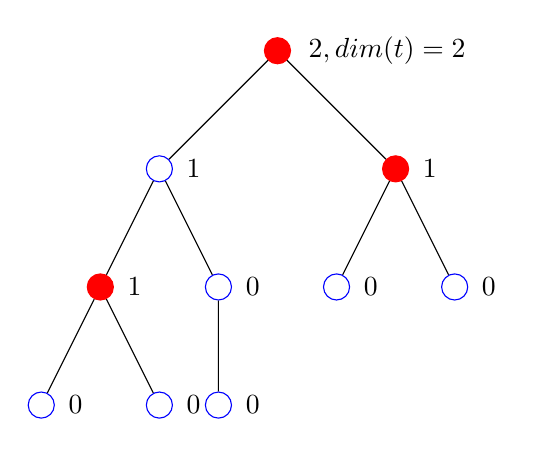
\begin{tikzpicture}[
level 1/.style={sibling distance=3cm},
level 2/.style={sibling distance=1.5cm}]
%\tikzstyle{every node}=[circle,draw]

\node[circle,draw] (Root) [ fill=red, red] {}
    child {
    node[circle,draw, blue] (l) {} 
    child { node[circle,draw, fill=red, red](ll) {}
            child { node[circle,draw, blue] (p) {} }
            child { node[circle,draw, blue] (pl) {} }
             }
    child { node[circle,draw, blue](lr) {} 
          child { node[circle,draw, blue] (plr) {} }
      }
}
child {
    node[circle,draw,  fill=red, red] (r) {}
    child { node[circle,draw, blue] (rl) {}} 
    child { node[circle,draw, blue] (rr) {} }
};
\node  [right=0.05cm of p] {0};
\node  [right=0.1cm of Root] {$2, dim(t)=2$};
\node  [right=0.05cm of l] {1};
\node  [right=0.05cm of r] {1};
\node  [right=0.05cm of ll] {1};
\node  [right=0.05cm of lr] {0};
\node  [right=0.05cm of pl] {0};
\node  [right=0.05cm of plr] {0};
\node  [right=0.05cm of rl] {0};
\node  [right=0.05cm of rr] {0};
\end{tikzpicture}
\caption{A tree $t$ with $dim(t)=2$. Nodes having children without unique maximum are filled.}
\label{oscbtree}            
\end{figure}


It is known that the dimension of parse trees and its oscillation are in linear relationship.

\begin{lemma}[\cite{BoundOsc}]
\label{boscdim}
Let a grammar $G = (\Sigma, N, P, S)$ be in Chomsky normal form and let $t$ be a parse tree of $G$. Then $osc(t) - 1 \le dim(t) \le 2osc(t)$.
\end{lemma}
\paragraph{Context-free language reachability.} 
A \textit{directed labeled graph} is a triple $D = (Q, \Sigma, \delta)$, where $Q$ is a finite set of nodes, $\Sigma$ is a finite set of alphabet symbols,
and $\delta \subseteq Q \times \Sigma \times Q$ is a finite set of labeled edges. Let $L(D)$ denote a graph language~--- a regular language, which is recognized by the NFA $(Q,\Sigma ,\delta ,Q, Q)$ obtained from $D$ by setting every state as inial and accepting.


Let $i\pi j$ denote a unique path between nodes $i$ and $j$ of the input graph and $l(\pi)$ denote a unique string obtained by concatenating edge labels along the path $\pi$. Then the CFL-reachability can be defined as follows.
\begin{definition}[Context-free language reachability]
Let $L \subseteq \Sigma^*$ be a context-free language and $D = (Q, \Sigma, \delta)$ be a directed labeled graph. Given two nodes $i$ and $j$ we say that $j$ is \textit{reachable} from $i$ if there exists a path $i \pi j$, such that $l(\pi) \in L$. 
\end{definition}
There are four varieties of CFL-reachability problems: all-pairs problem, single-source problem, single-target problem and single-source/single-target problem \cite{RepsBasic}. In this paper we consider all-pairs problem. The \textit{all-pairs problem} is to determine all pairs of nodes $i$ and $j$ such that $j$ is reachable from $i$. 




\section{CFPQ on planar digraphs}

We want to consider algorithms for semi-dynamic transitive closure for the case of a planar graph. Our algorithm needs to support only edge insertions that do not violate planarity.

There are several algorithms that look into the problem of dynamic reachability in planar digraphs and have sublinear both update and query time~\cite{10.5555/647903.739284},~\cite{karczmarz2018data},~\cite{kao2008encyclopedia}. 

Some algorithms~\cite{10.5555/1778580.1778635},~\cite{karczmarz2018data} restrict insertions to only that edges that respect the specific embedding of the planar graph. 

\todo[inline]{maybe we can choose one embedding at random and hope that nothing will violate it. So it will be monte-carlo (why it will have good probability? where from can we get all the possible non-isomorphic embeddings?)}  

The algorithms that allow edge insertions not with respect to the embedding of the graph, but to the planarity, are described in~\cite{10.5555/647903.739284},~\cite{10.1145/300515.300517}. The main idea of both articles is the same: a planar graph is separated into \textit{clusters} (edge induced subgraphs) for which reachability is shown by their sparse substitute $S$. \textit{Sparse substitute} is a graph that contains the reachability information between some set of vertices that lie in the same face of an embedded graph.

We show the results of~\cite{10.5555/647903.739284} more closely as they differ from the results of~\cite{10.1145/300515.300517} only by a logarithmic factor, have the same idea and are easier for understanding. 

Updates and queries are the following: adding or deleting the edge between vertices $u, v$, checking reachability, checking if new edge $(u, v)$ violates planarity. 

Every update procedure modifies a constant number of clusters, for which we reconstruct their sparse substitutes. If the procedure added the edge, new edge forms its own cluster. Moreover after every $\mathcal{O}(n^{1/3})$ insertions we rebuild cluster partition and sparse substitutes from the scratch so that clusters do not lose their properties, this rebuilding time is distributed between these $\mathcal{O}(n^{1/3})$ insertions, so insertion time is amortized. 

After splitting graph into clusters and looking into its sparse substitute update or query about vertices $u, v$ can be done by placing clusters of the vertices $u, v$ in the original graph $G$ into the graph of sparse substitutes $S$.

For maintaining dynamic transitive closure in this way we only need planarity to divide graph $G$ into clusters and for each cluster to build its sparse substitute. As we rebuild cluster partition and substitutes at the beginning and after every $\mathcal{O}(n^{\frac{1}{3}})$ edge-insertions, graph needs to remain planar during the updates. 

The results are the following.
 
\begin{enumerate}
	\item The amount of time for preprocessing is $\mathcal{O}(n \log n)$ --- in this time we find the separation of the given graph $G$ into $\mathcal{O}(n^{\frac{1}{3}})$ clusters (each consists of no more than $n^{\frac{2}{3}}$ edges of $G$) and build sparse substitution graph $S$ of total size $\mathcal{O}(n^{\frac{2}{3}} \log n)$ for them.
	
	\item After that we can perform add operation in $\mathcal{O}(n^{\frac{2}{3}} \log n)$ amortized time, delete operation in $\mathcal{O}(n^{\frac{2}{3}} \log n)$ worst-case time.
	
	\item Reachability query takes $\mathcal{O}(n^{\frac{2}{3}} \log n)$ worst-case time.
	
	\item Checking if the graph is planar can be done in $\mathcal{O}(n^{\frac{1}{2}})$ amortized time. 
\end{enumerate}

Let us look closely on how can we use the power of sparse substitution on our incremental transitive closure problem.

\begin{proposition}
We can maintain the structure described in~\cite{10.5555/647903.739284} not only for planar graphs, but for planar graphs with $\mathcal{O}(n^{\frac{1}{3}})$ edges that violate planarity. 
\end{proposition}

$\square$
In~\cite{10.5555/647903.739284} the number of clusters is $\mathcal{O}(n^{\frac{1}{3}})$. In the beginning and after every $\mathcal{O}(n^{\frac{1}{3}})$ edge insertions we rebuild sparse substitute graph $S$. and in these moments we need planarity. We can additionally maintain the set of non-planar edges, each edge of this set will present its own cluster and will not take part in the rebuilding of sparse substitution. Edge is \textit{non-planar} if its insertion to current planar graph $G$ makes it non-planar.
$\hfill\blacksquare$

\begin{proposition}
We can add edges in the graph and print out new pairs of reachable vertices for every insertion in $\mathcal{O}(n^{\frac{5}{3}})$ total time for every sequence of insertions if our model allows parallel computations.
\end{proposition}

$\square$
From~\cite{10.5555/647903.739284} we can add an edge $(u, v)$ in $\mathcal{O}(n^{\frac{2}{3}}\log n)$ amortized time. We want to get all pairs of vertices that are connected through the new edge.

We can run DFS from $v$ and DFS on reversed edges from $u$ in graph $S$ of sparse substitutes. DFS runs in time proportional to the size of the graph $S$ --- $\mathcal{O}(n^{\frac{2}{3}} \log n)$. After that for every cluster in the original graph $G$ we create dummy vertex $s$ and edges from $s$ to all boundary vertices in the cluster that were reached from $u$ and $v$ respectively. Then run DFS from this dummy vertex $s$. We print out every vertex that was reached by our DFSs, so we get two lists $U$ and $V$ for beginnings and the endings of the paths, going through $(u, v)$.

If any vertex $w$ is reachable from $v$ (without loss of generation), then it is a boundary vertex or lie in some cluster and is reachable from some boundary vertex of this cluster. In both cases, one of DFS's will print it out and the algorithm is correct. 

If we can run these DFS's in parallel (there are $\mathcal{O}(n^{\frac{1}{3}})$ clusters and the same number of DFS's), then each of them will take $\mathcal{O}(n^{\frac{2}{3}})$ amount of time (all cluster have $\mathcal{O}(n^{\frac{2}{3}})$ edges by definition in~\cite{10.5555/647903.739284}). As maximum number of edges in the planar graph is linear, the total amount of time will be $\mathcal{O}(n^{\frac{5}{3}})$ for every sequence of edge insertions.
$\hfill\blacksquare$

\begin{conjecture}
If our model does not allow parallel computations total amount of time for every sequence of insertions is at most $\mathcal{O}(n^2)$ and planarity does not get us any advantage in solving the problem of dynamic reachability (in amortized time per edge and query).
\end{conjecture}

[Thoughts]
If our model can not run algorithms in parallel, then the amount of time taken by iterating DFS's described above for every cluster is linear --- $\mathcal{O}(n)$. This means that usual DFS on the original graph $G$ has the same complexity and we will spend in total $\mathcal{O}(n^2)$ time.
$\hfill\blacksquare$

\todo[inline]{maybe we can spare some space ($\mathcal{O}(n^2)$?) so we can store list of reachable vertices from any boundary vertex and somehow update them during the edge additions?}

\section{Conclusion}

Conclusion, current state, results.

Future work. Library extension up to full GraphBLAS API implementation.

LaGraph on F\# .NET.

Evaluation. Comparison with other implementations on different devices.
Manual implementation versus translation.  

Another direction of future work is Brahma.FSharp improvements. 
First of all, it is necessary to support discriminated unions to make it possible to express custom semirings such as \texttt{Min-Plus}, as presented in listing~\ref{lst_example}. 

Also, it is necessary to add high-level abstractions for asynchronous programming, and for multi-GPU programming.
Such mechanisms can be naturally expressed in F\# with native primitives for asynchronous programming.

fusion and other optimizations.



%%
%% The next two lines define the bibliography style to be used, and
%% the bibliography file.
\bibliographystyle{ACM-Reference-Format}
\bibliography{references}

\end{document}
\endinput
%%
%% End of file `sample-sigconf.tex'.
